\documentclass[12pt]{article}

% Paquetes básicos primero
\usepackage[utf8]{inputenc}
\usepackage[T1]{fontenc}
\usepackage{ragged2e}
\usepackage[spanish]{babel}
\usepackage{siunitx}

% Geometría y diseño
\usepackage{geometry}
\geometry{
	letterpaper,
	left=2.5cm,
	right=2.5cm,
	top=3cm,
	bottom=3cm,
	headheight=60pt,
	headsep=1cm
}

% Paquetes de formato
\usepackage{setspace}
\usepackage{graphicx}
\usepackage{fancyhdr}
\usepackage{xcolor}
\usepackage{tcolorbox}
\usepackage{enumitem}
\usepackage{lastpage}
\usepackage{background}

\usepackage{listings}
\usepackage{inconsolata}
\usepackage{fontawesome}
\usepackage{mdframed}

% Definición de colores para código
\definecolor{lightgray}{gray}{0.95}
\definecolor{darkgray}{gray}{0.3}
\definecolor{mediumgray}{gray}{0.6}

% Estilo para cajas de comando
\newtcolorbox{comando}[1]{
	colback=lightgray,
	colframe=black,
	boxrule=0.5pt,
	arc=2pt,
	title={\faTerminal\ #1},
	fontupper=\ttfamily,
	before skip=10pt,
	after skip=10pt,
	left=5pt,
	right=5pt,
	top=5pt,
	bottom=5pt
}

% Configuración de listings
\lstset{
	basicstyle=\ttfamily\small,
	backgroundcolor=\color{lightgray},
	frame=single,
	framesep=3pt,
	breaklines=true,
	breakatwhitespace=true,
	showstringspaces=false,
	numbers=left,
	numberstyle=\tiny\color{darkgray},
	numbersep=8pt,
	keywordstyle=\color{black}\bfseries,
	commentstyle=\color{mediumgray},
	stringstyle=\color{black},
	captionpos=b,
	framerule=0.5pt,
	rulecolor=\color{black}
}

% Definición de entorno para notas
\newmdenv[
linewidth=0.5pt,
linecolor=black,
topline=false,
rightline=false,
bottomline=false,
leftmargin=10pt,
innerleftmargin=5pt,
skipabove=10pt,
skipbelow=10pt
]{nota}

% Paquetes para referencias
\usepackage[round]{natbib}  % Configuración específica para citas
\bibliographystyle{plainnat}  % Estilo de bibliografía

% URLs y enlaces (hyperref debe ir al final)
\usepackage{url}
\usepackage[hidelinks]{hyperref}

% Configuración del encabezado y pie de página
\pagestyle{fancy}
\fancyhf{}
\renewcommand{\headrulewidth}{0pt}
\renewcommand{\footrulewidth}{0pt}

\definecolor{tecnmBlue}{RGB}{0, 43, 89}
\definecolor{tecnmWhite}{RGB}{255, 255, 255}

% Definir comandos para reducir la carga
\newcommand{\smallgray}[1]{{\scriptsize\textcolor{gray}{#1}}}

\fancyhead[L]{%
	\hspace*{0.5cm}\raisebox{-2.2\height}{
\includegraphics[height=1cm]{imagenes/logotecnm.png}}%
}

\fancyhead[R]{%
	\raisebox{-1.7\height}{%
		\begin{tabular}[b]{r}
			{\scriptsize\textbf{Instituto Tecnológico de Morelia}}\\[-0.6em]
			\smallgray{Subdirección Académica}\\[-0.6em]
			\smallgray{Departamento de Sistemas y Computación}\\[-0.6em]
			\smallgray{Internet de todas las cosas}\\[-0.4em]
			{\scriptsize Página \thepage\ de \pageref{LastPage}}
		\end{tabular}%
	}%
}

\makeatletter
\renewcommand\@biblabel[1]{#1.}
\makeatother

\fancyfoot[L]{%
	\small
	Sensor Infrarojo (deteccion movimiento)
	
	\vspace{0.1cm}
	
	\small\textcolor{gray}{Luis Fernando Chávez Martínez}
	
	\vspace{0.1cm}
	
	\small\textcolor{gray}{Mario Eduardo Sánchez Mejía}
	
}
\fancyfoot[R]{%
	\small
	~
	
	\vspace{0.1cm}
	
	\textbf{21120187}%
	
	\vspace{0.1cm}
	
	\textbf{21120721}%
	
}
% Definir comando para citas
\newcommand{\cita}[1]{\cite{#1}}

\begin{document}
	\pagenumbering{arabic}
	
	
	% Secciones principales
	% portada.tex
% Configuración del fondo solo para la portada
\backgroundsetup{
	scale=1,
	angle=0,
	opacity=0.2,
	contents={
\includegraphics[width=\paperwidth,height=\paperheight]{imagenes/fondo_portada.png}}
}
\BgThispage

\begin{center}
	\vspace*{2cm}
	
	\Large\textbf{Tarea 2: Primera Extracción de Datos}
	
	\vspace{1.5cm}
	
	Autor(es):
	
	\vspace{0.5cm}
	
	Luis Fernando Chávez Martínez
	
	Mario Eduardo Sánchez Mejía
	
	
	\vspace{1.5cm}
	
	Docente:
	
	\vspace{0.5cm}
	
	
	Aurelio Amaury Coria Ramirez
	
	\vspace{0.5cm}
	
	\begin{abstract}
		\noindent
		\justifying
		La presente investigación aborda el desarrollo de una alternativa de código abierto a las plataformas comerciales de Business Intelligence, centrándose específicamente en replicar las funcionalidades principales de Power BI utilizando Python. Se analiza la arquitectura necesaria para implementar un sistema completo de análisis y visualización de datos, identificando los componentes críticos para el procesamiento, análisis y presentación de información. La investigación examina las diferentes tecnologías y frameworks disponibles para cada componente del sistema, desde la extracción y transformación de datos hasta la visualización interactiva y el despliegue en producción. Este estudio contribuye al campo de la analítica de datos proporcionando un marco de trabajo para la implementación de soluciones personalizadas de Business Intelligence, beneficiando a organizaciones que requieren mayor flexibilidad y control sobre sus herramientas de análisis de datos. \\
		
		\textbf{Palabras clave:} ETL, Visualización de datos, Python, Desarrollo web, Bases de datos, Machine Learning, DevOps, Dashboards interactivos, Análisis de datos, Interfaz de usuario, Business Intelligence, Código abierto.
	\end{abstract}
\end{center}

% Desactivar el fondo para las siguientes páginas
\clearpage
\backgroundsetup{contents={}}
	
	
	\tableofcontents
	\newpage
	\section{Introducción}
\noindent
\justifying
En la era actual de la transformación digital, la capacidad de analizar y visualizar datos de manera efectiva se ha convertido en una necesidad fundamental para las organizaciones. Las herramientas de Business Intelligence (BI) comerciales, como Power BI, han dominado el mercado, ofreciendo soluciones robustas pero a menudo limitadas por su naturaleza propietaria y costos asociados. Esta realidad plantea un desafío significativo para organizaciones que buscan mayor flexibilidad, personalización y control sobre sus procesos de análisis de datos.
El ecosistema de Python, con su rica biblioteca de herramientas de código abierto, presenta una oportunidad única para desarrollar alternativas viables a estas soluciones comerciales. Sin embargo, la implementación de un sistema completo de BI requiere una comprensión profunda de múltiples componentes y tecnologías, desde la gestión de datos hasta la visualización interactiva.
Esta investigación se centra en explorar y documentar la arquitectura necesaria para construir una plataforma de BI utilizando Python, abordando los desafíos técnicos y consideraciones de diseño que surgen en el proceso. El estudio no solo examina las tecnologías individuales disponibles, sino que también analiza cómo estas pueden integrarse efectivamente para crear un sistema cohesivo y funcional.
La relevancia de esta investigación se fundamenta en tres aspectos principales: primero, la creciente necesidad de soluciones de BI personalizables y escalables; segundo, la tendencia hacia la adopción de tecnologías de código abierto en entornos empresariales; y tercero, la importancia de democratizar el acceso a herramientas avanzadas de análisis de datos.
Este trabajo busca contribuir al campo del análisis de datos proporcionando un marco de referencia para desarrolladores y organizaciones que desean implementar sus propias soluciones de BI. La investigación no solo aborda aspectos técnicos, sino que también considera factores prácticos como la escalabilidad, mantenibilidad y seguridad, elementos cruciales para cualquier implementación en un entorno de producción.
	\newpage
	\section{Desarrollo Experimental}
El desarrollo del detector de movimiento con sensor infrarrojo PIR (HC-SR501) se llevó a cabo siguiendo una metodología estructurada que incluyó el montaje del circuito, la configuración del sensor y la programación del sistema de control.

\subsection{Materiales}
Para la implementación del proyecto se utilizaron los siguientes componentes:
\begin{itemize}
	\item Raspberry Pi (con 40 pines GPIO)
	\item Placa de expansión GPIO y cable plano
	\item Protoboard
	\item 5 cables puente
	\item Sensor HC-SR501 (sensor PIR)
	\item 1 LED
	\item 1 Resistencia de \SI{220}{\ohm}
\end{itemize}

\subsection{Montaje del Circuito}
El circuito fue ensamblado de acuerdo con el esquema proporcionado en la práctica. La conexión del sensor PIR a la Raspberry Pi se realizó considerando los siguientes aspectos:

\begin{enumerate}
	\item El sensor HC-SR501 se alimentó con 5V desde la Raspberry Pi.
	\item La salida del sensor se conectó al pin GPIO 0 (según la numeración de WiringPi).
	\item El LED indicador se conectó al pin GPIO 1 con una resistencia limitadora de corriente de \SI{220}{\ohm}.
\end{enumerate}

Es importante destacar que el sensor PIR requiere aproximadamente un minuto de inicialización después de ser alimentado, durante el cual puede alternar entre niveles altos y bajos de salida sin relación con la detección de movimiento.

\subsection{Configuración del Sensor}
Previo a la implementación del código, se configuró el sensor PIR ajustando los dos potenciómetros disponibles:

\begin{enumerate}
	\item R1: Se ajustó para establecer el tiempo de retardo de la señal de salida después de detectar movimiento. Para esta práctica, se configuró en un valor intermedio proporcionando un retardo de aproximadamente 5-7 segundos.
	\item R2: Se ajustó para determinar la distancia máxima de detección. Se calibró para detectar movimiento en un rango de aproximadamente 3 metros.
\end{enumerate}

Adicionalmente, se configuró el puente selector en posición "L" para utilizar el modo de disparo no repetitivo, lo que significa que después de detectar movimiento y emitir un nivel alto, el sensor no detectará nuevos movimientos hasta que finalice el tiempo de retardo establecido.

\subsection{Implementación del Software}
El programa para controlar el sistema fue desarrollado en lenguaje C utilizando la biblioteca WiringPi para la interacción con los pines GPIO de la Raspberry Pi. El algoritmo implementado sigue un enfoque simple:

\begin{enumerate}
	\item Configuración de los pines GPIO 0 (sensor) como entrada y GPIO 1 (LED) como salida.
	\item Implementación de un bucle infinito que constantemente verifica el estado del sensor.
	\item Cuando el sensor detecta movimiento, emite un nivel alto que es leído por el programa.
	\item En respuesta a la detección, el LED se enciende y se muestra un mensaje en la terminal.
	\item Cuando no se detecta movimiento, el LED se apaga y se actualiza el mensaje en la terminal.
\end{enumerate}

El código fue compilado y ejecutado utilizando los siguientes comandos:
\begin{verbatim}
	gcc SenseLED.c -o SenseLED -lwiringPi
	sudo ./SenseLED
\end{verbatim}

\section{Resultados}
Los resultados del experimento se documentaron mediante capturas fotográficas que ilustran el funcionamiento del sistema en diferentes situaciones. A continuación, se presentan las imágenes que muestran el comportamiento del detector de movimiento implementado.

\begin{figure}[h]
	\centering
	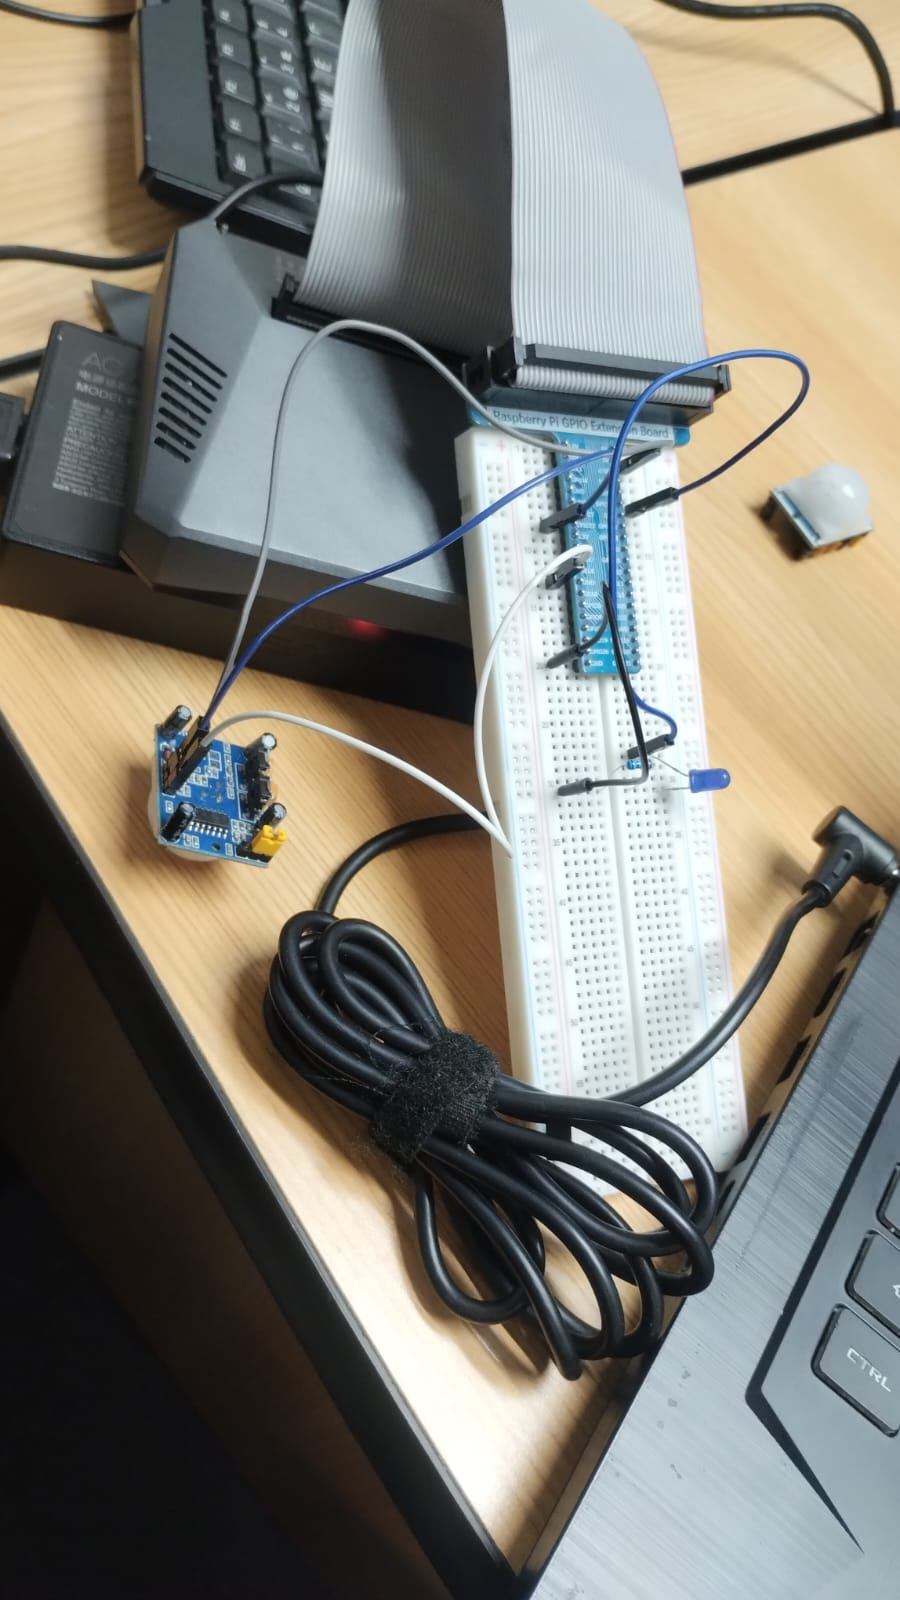
\includegraphics[width=0.5\textheight]{imagenes/1.jpg}
	\caption{Montaje completo del circuito con Raspberry Pi, protoboard, sensor PIR y LED.}
	\label{fig:circuito}
\end{figure}

\begin{figure}[h]
	\centering
	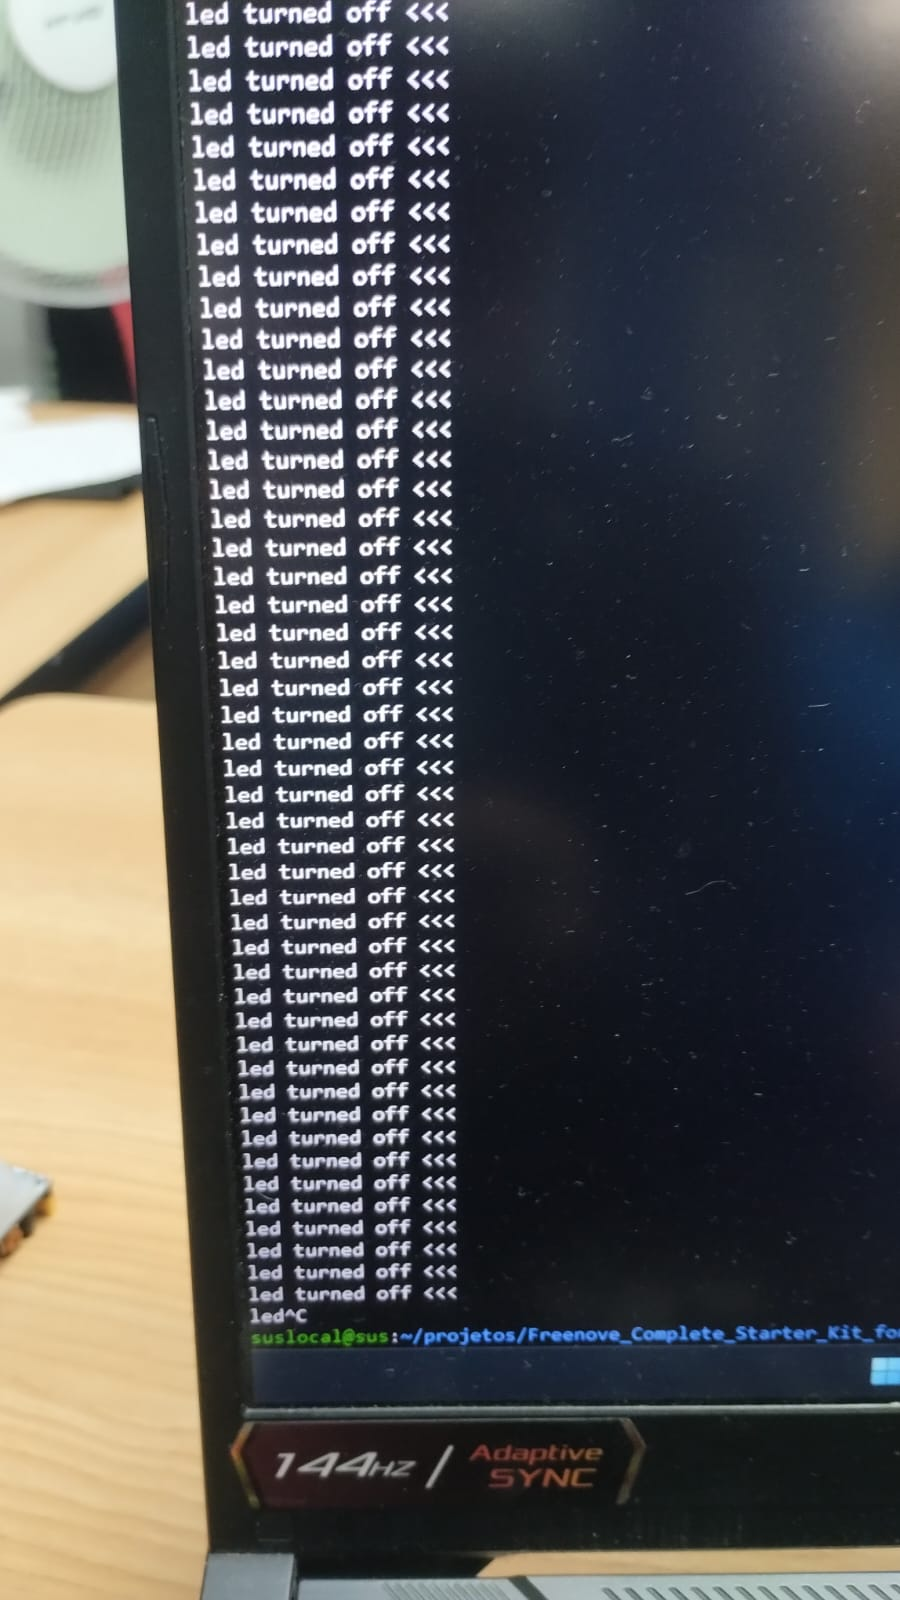
\includegraphics[width=0.5\textheight]{imagenes/2.jpg}
	\caption{Salida en terminal mostrando los mensajes de estado durante la ejecución del programa.}
	\label{fig:terminal}
\end{figure}

\begin{figure}[h]
	\centering
	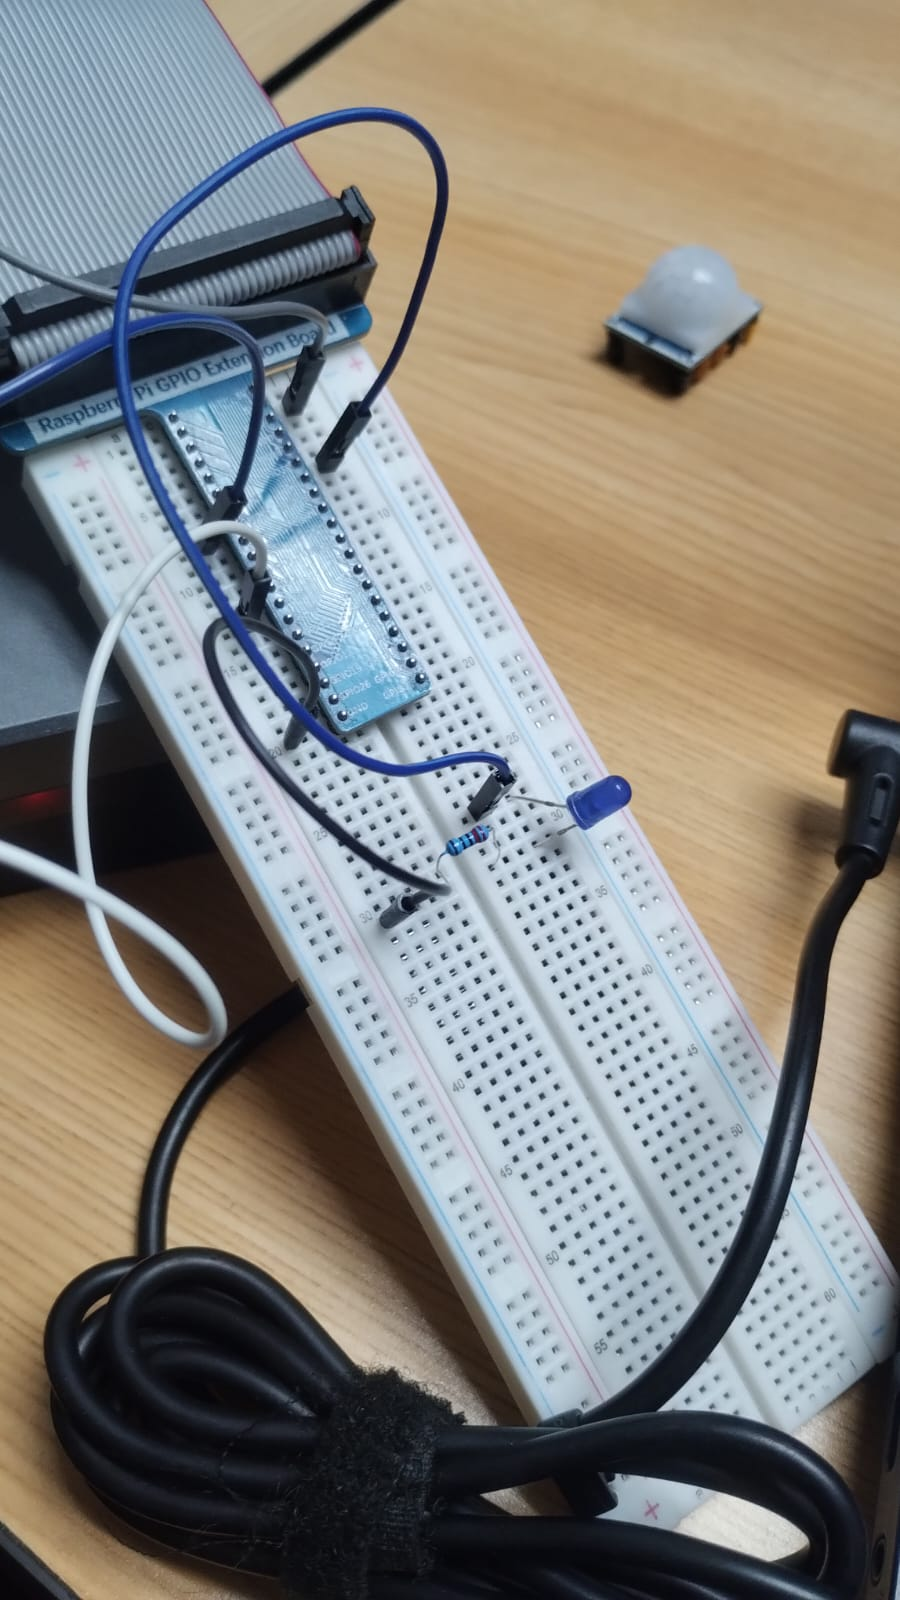
\includegraphics[width=0.5\textheight]{imagenes/3.jpg}
	\caption{Sistema en funcionamiento con LED apagado indicando sin detección de movimiento.}
	\label{fig:deteccionOFF}
\end{figure}

\begin{figure}[h]
	\centering
	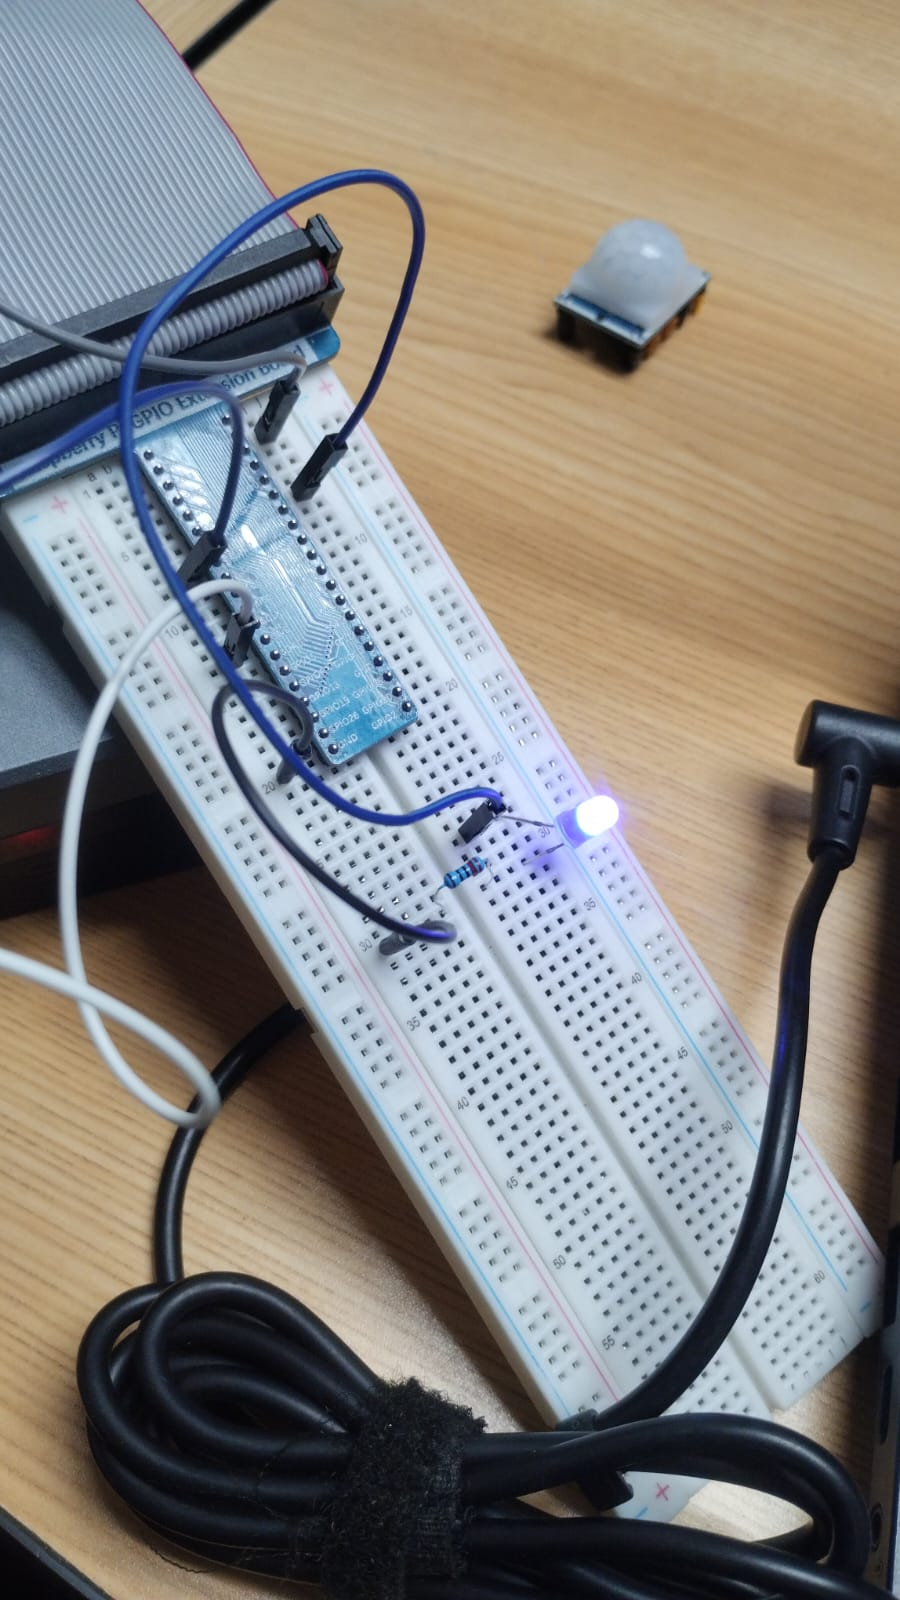
\includegraphics[width=0.5\textheight]{imagenes/4.jpg}
	\caption{Sistema en funcionamiento con LED encendido indicando detección de movimiento.}
	\label{fig:detenccionON}
\end{figure}

Las imágenes ilustran claramente el funcionamiento del sistema de detección de movimiento, mostrando tanto la configuración física como la respuesta del sistema. Se puede observar que el LED se enciende efectivamente cuando se detecta movimiento y se apaga cuando no hay actividad dentro del rango de detección del sensor.
	\newpage
	\section{Conclusión}

En esta actividad logramos implementar un circuito básico de encendido y apagado de un LED mediante un botón utilizando una Raspberry Pi. A lo largo del desarrollo, comprendimos la importancia de las resistencias pull-down para evitar estados indeterminados en la entrada digital y reforzamos el uso de los pines GPIO para la interacción con hardware externo.

Este ejercicio no solo permitió reforzar conceptos fundamentales de electrónica y programación, sino que también sirvió como base para futuros proyectos en los que se requiera el control de dispositivos a través de una Raspberry Pi. Gracias a esta práctica, estamos mejor preparados para integrar componentes adicionales como sensores o actuadores, ampliando así las posibilidades de automatización y control en sistemas embebidos.

	
	% Referencias
	%\clearpage
	%\addcontentsline{toc}{section}{Referencias}
	%\bibliography{referencias} 
	
\end{document}